\documentclass[letterpaper,fleqn,leqno]{article}

\usepackage{amsmath}
\usepackage{amssymb}
\usepackage{enumerate}
\usepackage[letterpaper, margin=1in]{geometry}
\usepackage{xcolor, colortbl}
\usepackage{tabularx}
\usepackage{tikz}

\setlength{\extrarowheight}{3pt}

\begin{document}
	\newcommand{\problem}[1]{\noindent\textbf{Problem #1.}}
	\newcommand{\chunk}[1]{
		\noindent\begin{minipage}[t]{\textwidth}
			#1
		\end{minipage}
	}
	\newcommand{\ques}[3]{
		\begin{enumerate}
			\item [#1] #2 \\
			#3
		\end{enumerate}
	}
	\newcommand{\quesa}[3]{
		\begin{enumerate}
			\item [(#1)] #2 \\
			#3
		\end{enumerate}
	}
	\newcommand{\set}[4]{
		\quesa{#3}{Exercise Set 5.#1, Problem #2}{#4}
	}
	\newcommand{\sets}[4]{
		\quesa{#3}{Exercise Set 5.#1, Problems #2}{#4}
	}

	\newcommand{\Sum}[2]{\displaystyle\sum\limits_{#1}^{#2}}
	\newcommand{\Prod}[2]{\displaystyle\prod\limits_{#1}^{#2}}

	\newcommand{\qeq}{\stackrel{?}{=}}
	\newcommand{\qg}{\stackrel{?}{>}}
	\newcommand{\ql}{\stackrel{?}{<}}
	\newcommand{\qgeq}{\stackrel{?}{\geq}}
	\newcommand{\qleq}{\stackrel{?}{\leq}}

	\newcommand{\case}[2]{\cellcolor{yellow!25}\textbf{Case #1:} #2}

	\chunk{
		\problem{1}
		\set{2}{11}{a}{
			$1^3+2^3+\dots+n^3=\left[\dfrac{n(n+1)}{2}\right]^2$, for all integers $n\geq1$. \\
			Let property $P(n)$ be $\Sum{i=1}{n} i^3=\left[\dfrac{n(n+1)}{2}\right]^2$. \\
			\textbf{Basis:} \\
			$P(1): \left(\Sum{i=1}{1} i^3=1\right)=\left(\left[\dfrac{n(n+1)}{2}\right]^2=1\right)$ is true. \\
			\textbf{Inductive hypothesis:} \\
			Assume $P(k): \Sum{i=1}{k} i^3=\left[\dfrac{k(k+1)}{2}\right]^2$ for $k\geq1\in\mathbb{Z}$ is true. \\
			Prove $P(k+1): \Sum{i=1}{k+1} i^3=\left[\dfrac{(k+1)(k+2)}{2}\right]^2$: \\
			$\begin{aligned}[t]
				\Sum{i=1}{k+1} i^3 &\qeq \left[\dfrac{(k+1)(k+2)}{2}\right]^2 \\
				\left(\Sum{i=1}{k}i^3\right)+(k+1)^3 &\qeq \left[\dfrac{k^2+3k+2}{2}\right]^2 \\
				\left[\dfrac{k(k+1)}{2}\right]^2+k^3+3k^2+3k+1 &\qeq \left[\dfrac{k^2+3k+2}{2}\right]^2 \\
				\left[\dfrac{k^2+k}{2}\right]^2+k^3+3k^2+3k+1 &\qeq \left[\dfrac{k^2+3k+2}{2}\right]^2 \\
				\dfrac{k^4+2k^3+k^2}{4}+\dfrac{4k^3+12k^2+12k+4}{4} &\qeq \dfrac{k^4+3k^3+2k^2+3k^3+9k^2+6k+2k^2+6k+4}{4} \\
				\dfrac{k^4+6k^3+13k^2+12k+4}{4} &= \dfrac{k^4+6k^3+13k^2+12k+4}{4} \\
			\end{aligned}$ \\
			Basis and inductive hypothesis proven, therefore original statement is true. \\
		}
	}
	\chunk{
		\set{2}{14}{b}{
			$\Sum{i=1}{n+1}i\cdot2^i=n\cdot2^{n+2}+2$, for all integers $n\geq0$. \\
			Let property $P(n)$ be $\Sum{i=1}{n+1}i\cdot2^i=n\cdot2^{n+2}+2$. \\
			\textbf{Basis:} \\
			$P(0): \left(\Sum{i=1}{1}i\cdot2^i=2\right)=\left(0\cdot2^{2}+2=2\right)$ is true. \\
			\textbf{Inductive hypothesis:} \\
			Assume $P(k): \Sum{i=1}{k+1}i\cdot2^i=k\cdot2^{k+2}+2$ for $k\geq0\in\mathbb{Z}$ is true. \\
			Prove $P(k+1): \Sum{i=1}{k+2}i\cdot2^i=(k+1)\cdot2^{k+3}+2$: \\
			$\begin{aligned}[t]
				\Sum{i=1}{k+2}i\cdot2^i &\qeq (k+1)\cdot2^{k+3}+2 \\
				\left(\Sum{i=1}{k+1}i\cdot2^i\right) + (k+2)\cdot2^{k+2} &\qeq (k+1)\cdot2^{k+3}+2 \\
				k\cdot2^{k+2}+2+(k+2)\cdot2^{k+2} &\qeq (k+1)\cdot2^{k+3}+2 \\
				k\cdot2^{k+2}+2+k\cdot2^{k+2}+2^{k+3} &\qeq (k+1)\cdot2^{k+3}+2 \\
				2k\cdot2^{k+2}+2+2^{k+3} &\qeq (k+1)\cdot2^{k+3}+2 \\
				k\cdot2^{k+3}+2+2^{k+3} &\qeq (k+1)\cdot2^{k+3}+2 \\
				(k+1)\cdot2^{k+3}+2 &= (k+1)\cdot2^{k+3}+2 \\
			\end{aligned}$ \\
			Basis and inductive hypothesis proven, therefore original statement is true. \\
		}
	}
	\chunk{
		\set{2}{17}{c}{
			$\Prod{i=0}{n}\left(\dfrac{1}{2i+1}\cdot\dfrac{1}{2i+2}\right)=\dfrac{1}{(2n+2)!}$, for all integers $n\geq0$. \\
			Let property $P(n)$ be $\Prod{i=0}{n}\left(\dfrac{1}{2i+1}\cdot\dfrac{1}{2i+2}\right)$. \\
			\textbf{Basis:} \\
			$P(0): \left(\Prod{i=0}{0}\left(\dfrac{1}{2i+1}\cdot\dfrac{1}{2i+2}\right)=\dfrac{1}{2}\right)=\left(\dfrac{1}{(0+2)!}=\dfrac{1}{2}\right)$ is true. \\
			\textbf{Inductive Hypothesis:} \\
			Assume $P(k): \Prod{i=0}{k}\left(\dfrac{1}{2i+1}\cdot\dfrac{1}{2i+2}\right)=\dfrac{1}{(2k+2)!}$ for $k\geq0\in\mathbb{Z}$ is true. \\
			Prove $P(k+1): \Prod{i=0}{k+1}\left(\dfrac{1}{2i+1}\cdot\dfrac{1}{2i+2}\right)=\dfrac{1}{(2(k+1)+2)!}$: \\
			$\begin{aligned}[t]
				\Prod{i=0}{k+1}\left(\dfrac{1}{2i+1}\cdot\dfrac{1}{2i+2}\right) &\qeq \dfrac{1}{(2(k+1)+2)!} \\
				\Prod{i=0}{k}\left(\dfrac{1}{2i+1}\cdot\dfrac{1}{2i+2}\right)\left(\dfrac{1}{2(k+1)+1}\cdot\dfrac{1}{2(2k+1)+2}\right) &\qeq \dfrac{1}{(2k+4)!} \\
				\dfrac{1}{(2k+2)!}\left(\dfrac{1}{2k+3}\cdot\dfrac{1}{2k+4}\right) &\qeq \dfrac{1}{(2k+4)!} \\
				\dfrac{1}{(2k+2)!(2k+3)(2k+4)} &\qeq \dfrac{1}{(2k+4)(2k+3)!} \\
				\dfrac{1}{(2k+4)(2k+3)(2k+2)!} &= \dfrac{1}{(2k+4)(2k+3)(2k+2)!} \\
			\end{aligned}$ \\
			Basis and inductive hypothesis proven, therefore original statement is true. \\
		}
	}
	\chunk{
		\set{3}{10}{d}{
			$n^3-7n+3$ is divisible by 3, for each integer $n\geq0$. \\
			Let property $P(n)$ be $n^3-7n+3$ is divisible by 3. \\
			\textbf{Basis:} \\
			$P(0): (0^3-7\cdot0+3=0)$ is divisible by 3 is true. \\
			\textbf{Inductive Hypothesis:} \\
			Assume $P(k): k^3-7k+3$ is divisible by 3 where $k\geq0\in\mathbb{Z}$ is true. \\
			Prove $P(k+1): (k+1)^3-7(k+1)+3$ is divisible by 3: \\
			$\begin{aligned}[t]
				& (k+1)^3-7(k+1)+3 \\
				={} & k^3+3k^2+3k+1-7k-7+3 \\
				={} & \underbrace{\left(k^3-7k+3\right)}_{m}+3k^2+3k+1-7 \\
			\end{aligned}$ \\
			$P(k)$ is true, therefore $m$ is a multiple of 3 and $m=3a$ for some integer $a$. \\
			$\begin{aligned}[t]
				={} & 3a+3k^2+3k-6 \\
				={} & 3\left(a+k^2+k-2\right) \\
			\end{aligned}$ \\
			Expression is a multiple of 3, therefore $(k+1)^3-7(k+1)+3$ is divisible by 3. \\
			Basis and inductive hypothesis proven, therefore original statement is true. \\
		}
	}
	\chunk{
		\set{3}{17}{e}{
			$1+3n\leq4^n$, for every integer $n\geq0$. \\
			Let property $P(n)$ be $1+3n\leq4^n$. \\
			\textbf{Basis:} \\
			$P(0): (1+3\cdot0=1)\leq(4^0=1)$ is true. \\
			\textbf{Inductive hypothesis:} \\
			Assume $P(k): 1+3k\leq4^k$ for $k\geq0\in\mathbb{Z}$ is true. \\
			Prove $P(k+1): 1+3(k+1) \leq 4^{k+1}$: \\
			$\begin{aligned}[t]
				1+3(k+1) &\qleq 4^{k+1} \\
				4+3k &\qleq 4^{k+1} \\
				(1+3k)+3 &\qleq 4^{k+1} \\
				4^k+3 &\qleq 4^{k+1} & \text{$P(k)$ is true}\\
				3 &\qleq 4^{k+1}-4^k \\
				3 &\qleq 4^k(4-1) \\
				3 &\qleq 3\cdot4^k \\
				1 &\leq 4^k \\
			\end{aligned}$ \\
			Last inequality holds true for all $k\geq0\in\mathbb{Z}$. \\
			Basis and inductive hypothesis proven, therefore original statement is true. \\
		}
	}
	\chunk{
		\set{3}{21}{f}{
			$\sqrt{n}<\dfrac{1}{\sqrt{1}}+\dfrac{1}{\sqrt{2}}+\dots+\dfrac{1}{\sqrt{n}}$, for all integers $n\geq2$. \\
			Let property $P(n)$ be $\sqrt{n}<\Sum{i=1}{n}\dfrac{1}{\sqrt{i}}$. \\
			\textbf{Basis:} \\
			$P(2):(\sqrt{2})<\left(\Sum{i=1}{2}\dfrac{1}{\sqrt{i}}=\dfrac{1}{\sqrt{1}}+\dfrac{1}{\sqrt{2}}=1+\dfrac{\sqrt{2}}{2}\right)$ is true. \\
			\textbf{Inductive hypothesis:} \\
			Assume $P(k):\sqrt{k}<\Sum{i=1}{k}\dfrac{1}{\sqrt{i}}$ for $k\geq2\in\mathbb{Z}$ is true. \\
			Prove $P(k+1): \sqrt{k+1} < \Sum{i=1}{k+1}\dfrac{1}{\sqrt{i}}$: \\
			$\begin{aligned}[t]
				\sqrt{k+1} &\ql \Sum{i=1}{k+1}\dfrac{1}{\sqrt{i}} \\
				\sqrt{k+1} &\ql \Sum{i=1}{k}\dfrac{1}{\sqrt{i}}+\dfrac{1}{\sqrt{k+1}} \\
				\sqrt{k+1} &\ql \sqrt{k}+\dfrac{1}{\sqrt{k+1}} & \text{$P(k)$ is true} \\
				\dfrac{k+1}{\sqrt{k+1}} &\ql \dfrac{\sqrt{k}\sqrt{k+1}+1}{\sqrt{k+1}} \\
				k+1 &\ql \sqrt{k}\sqrt{k+1}+1 \\
				\sqrt{k}\sqrt{k} &\ql \sqrt{k}\sqrt{k+1} \\
				k &\ql k+1 \\
				0 &< 1 \\
			\end{aligned}$ \\
			Basis and inductive hypothesis proven, therefore original statement is true. \\
		}
	}
	\chunk{
		\set{3}{22}{g}{
			$1+nx\leq(1+x)^n$, for all real numbers $x>-1$ and integers $n\geq2$. \\
			Let property $P(n)$ be $1+nx\leq(1+x)^n$ for all $x>-1\in\mathbb{R}$. \\
			\textbf{Basis:} \\
			$P(2): \begin{aligned}[t]
				& 1+2x\leq(1+x)^2 \\
				\Rightarrow{} & 1+2x\leq1+2x+x^2 \\
				\Rightarrow{} &0\leq x^2 \\
			\end{aligned}$
			is true. \\
			\textbf{Inductive hypothesis:} \\
			Assume $P(k):1+kx\leq(1+x)^k$ for $k\geq2\in\mathbb{Z}$ and $x>-1\in\mathbb{R}$ is true. \\
			Prove $P(k+1): 1+(k+1)x\leq(1+x)^{k+1}$: \\
			$\begin{aligned}[t]
				1+(k+1)x &\qleq (1+x)^{k+1} \\
				1+kx+x &\qleq (1+x)^{k+1} \\
				(1+x)^k+x &\qleq (1+x)^{k+1} \\
				x &\qleq (1+x)^k((1+x)-1) \\
				x &\qleq (1+x)^kx \\
			\end{aligned}$ \\
			\begin{tabular}{|l|}
				\hline
				\case{1}{$x=0$} \\
				\hline
				Prove $x\leq(1+x)^kx$: \\
				$0 \leq (1+0)^k\cdot0$ \\
				$0 \leq 0$ \\
				Proof done. \\
				\hline
				\case{2}{$x>0$} \\
				\hline
				Prove $x\leq(1+x)^kx$: \\
				\\
				\begin{tabular}{l|l}
					$\begin{aligned}[t]
						x &> 0 \\
						1 &< 1+x \\
						1^k &< (1+x)^k \\
						1 &< (1+x)^k \\
					\end{aligned}$ &
					$\begin{aligned}[t]
						x & \qleq (1+x)^kx \\
						1 & \qleq (1+x)^k \\
					\end{aligned}$ \\
				\end{tabular} \\
				\\
				$\begin{aligned}[t]
					& 1<(1+x)^k \\
					\therefore{} & 1\leq(1+x)^k \\
					\therefore{} & x\leq(1+x)^kx \\
				\end{aligned}$ \\
				Proof done. \\
				\hline
			\end{tabular}
			\begin{tabular}{|l|}
				\hline
				\case{3}{$-1<x<0$} \\
				\hline
				Prove $x\leq(1+x)^kx$: \\
				\\
				\begin{tabular}{l|l}
					$\begin{aligned}[t]
						0 &>& x &>-1 \\
						1 &>& 1+x &>0 \\
						1^k &>& (1+x)^k &>0^k \\
						1 &>& (1+x)^k &>0 \\
					\end{aligned}$ &
					$\begin{aligned}[t]
						x &\qleq (1+x)^kx \\
						1 & \qgeq (1+x)^k \\
					\end{aligned}$ \\
				\end{tabular} \\
				\\
				$\begin{aligned}[t]
					& 1>(1+x)^k \\
					\therefore{} & 1\geq(1+x)^k \\
					\therefore{} & x\leq(1+x)^kx \\
				\end{aligned}$ \\
				Proof done. \\
				\hline
			\end{tabular} \\
			$P(k+1)$ is true in all cases. \\
			Basis and inductive hypothesis proven, therefore original statement is true. \\
		}
	}
	\chunk{
		\set{3}{29}{h}{
			As each of a group of businesspeople arrives at a meeting, each shakes hands with all the other people present. Use mathematical induction to show that if $n$ people come to the meeting then $[n(n-1)]/2$ handshakes occur. \\
			If the set of businesspeople has size $n$, then the number of handshakes is $\displaystyle \binom{n}{2}$. \\
			For a set of 0 and 1 businesspeople, no handshakes occur. \\
			$\displaystyle \binom{n}{2}=\dfrac{n!}{2!(n-2)!}=\dfrac{n!}{2(n-2)!}$ \\
			Let property $P(n)$ be $\begin{cases}
				0=\dfrac{n(n-1)}{2} & \text{if $n=0,\, n=1$} \\
				\dfrac{n!}{2(n-2)!}=\dfrac{n(n-1)}{2} & \text{if $n\geq2$} \\
			\end{cases}$. \\
			\textbf{Basis:} \\
			$P(0):0=\left(\dfrac{0(0-1)}{2}=0\right)$ is true. \\
			$P(1):0=\left(\dfrac{1(1-1)}{2}=0\right)$ is true. \\
			$P(2): \left(\dfrac{2!}{2(2-2)!}=\dfrac{2}{2\cdot1}=1\right)=\left(\dfrac{2(2-1)}{2}=1\right)$ is true. \\
			\textbf{Inductive hypothesis:} \\
			Assume $P(k): \dfrac{k!}{2(k-2)!}=\dfrac{k(k-1)}{2}$ for $k\geq2\in\mathbb{Z}$ to be true. \\
			Prove $P(k+1): \dfrac{(k+1)!}{2((k+1)-2)!}=\dfrac{(k+1)((k+1)-1)}{2}$: \\
			$\begin{aligned}[t]
				\dfrac{(k+1)!}{2((k+1)-2)!} &\qeq \dfrac{(k+1)((k+1)-1)}{2} \\
				\dfrac{(k+1)k!}{2(k-1)!} &\qeq \dfrac{(k+1)k}{2} \\
				\dfrac{(k+1)k(k-1)!}{2(k-1)!} &\qeq \dfrac{(k+1)k}{2} \\
				\dfrac{(k+1)k}{2} &= \dfrac{(k+1)k}{2} \\
			\end{aligned}$ \\
			Basis and inductive hypothesis proven, therefore original statement is true. \\
		}
	}
	\chunk{
		\quesa{i}{Prove that in an $n$-sided regular polygon, where $n\geq3$, the number of diagonals is $n(n-3)/2$.}{
			The number of possible vertex pairs in an $n$-sided regular polygon is $\displaystyle \binom{n}{2}$, and $n$ of these vertex pairs are the edges of the polygon. The number of diagonals is $\displaystyle \binom{n}{2}-n$. \\
			$\displaystyle \binom{n}{2}-n=\dfrac{n!}{2!(n-2)!}-n=\dfrac{n!}{2(n-2)!}-n$ \\
			Let property $P(n)$ be $\dfrac{n!}{2(n-2)!}-n=\dfrac{n(n-3)}{2}$. \\
			\textbf{Basis:} \\
			$P(3): \left(\dfrac{3!}{2(3-2)!}-3=\dfrac{6}{2}-3=0\right)=\left(\dfrac{3(3-3)}{2}=0\right)$ is true. \\
			\textbf{Inductive hypothesis:} \\
			Assume $P(k): \dfrac{k!}{2(k-2)!}-k=\dfrac{k(k-3)}{2}$ for $k\geq3\in\mathbb{Z}$ to be true. \\
			Prove $P(k+1): \dfrac{(k+1)!}{2((k+1)-2)!}-(k+1)=\dfrac{(k+1)((k+1)-3)}{2}$: \\
			$\begin{aligned}[t]
				\dfrac{(k+1)!}{2((k+1)-2)!}-(k+1) &\qeq \dfrac{(k+1)((k+1)-3)}{2} \\
				\dfrac{(k+1)k!}{2(k-1)!}-k-1 &\qeq \dfrac{(k+1)(k-2)}{2} \\
				\dfrac{(k+1)k(k-1)!}{2(k-1)!}-k-1 &\qeq \dfrac{(k+1)(k-2)}{2} \\
				\dfrac{(k+1)k}{2}-\dfrac{2k+2}{2} &\qeq \dfrac{(k+1)(k-2)}{2} \\
				\dfrac{k^2+k-2k-2}{2} &\qeq \dfrac{k^2-k-2}{2} \\
				\dfrac{k^2-k-2}{2} &= \dfrac{k^2-k-2}{2} \\
			\end{aligned}$ \\
			Basis and inductive hypothesis proven, therefore original statement is true. \\
		}
	}
	\chunk{
		\quesa{j}{Prove that the number of permutations of the set $\left\{1,2,\dots,n\right\}$ with $n$ elements is $n!$, for natural number $n\geq1$. \\}{
			A set of $n=1$ elements has $1!=1$ permutation. \\
			Let property $P(n)$ be $\left\{1,2,\dots,n\right\}$ has $n!$ permutations. \\
			\textbf{Basis:} \\
			$P(1): \left\{1\right\}$ has $1!=1$ permutation is true. \\
			\textbf{Inductive hypothesis:} \\
			Assume $P(k): \left\{1,2,\dots,k\right\}$ has $k!$ permutations for $k\geq1\in\mathbb{Z}$ to be true. \\
			In order to create a permuted set $B_p$ of size $k+1$, one can insert $k+1$ into $A_p$, an arbitrary permutation of set $A$ of $k$ elements. \\
			This action is equivalent to permuting a set of size $k+1$. \\
			There are $k+1$ positions to insert such an element into $A_p$: $k$ positions before each element and one position after the last element of $A_p$. \\
			There are $k!$ possible $A_p$ made from $A$. \\
			($k+1$ ways to insert into $A_p$) $\times$ ($k!$ possible $A_p$) = $(k+1)k! = (k+1)!$ ways to create $B_p$. \\
			$P(k+1)$ is true. \\
			Basis and inductive hypothesis proven, therefore original statement is true. \\
		}
	}

	\chunk{
		\problem{2}
		\set{4}{8}{a}{
			Suppose that $h_0,h_1,h_2,\dots$ is a sequence defined as follows: \\
			$h_0=1$, $h_1=2$, $h_2=3$, \\
			$h_k=h_{k-1}+h_{k-2}+h_{k-3}$ for all integers $k\geq3$.
			\begin{enumerate}[(a)]
				\item
				Prove that $h_n\leq3^n$ for all integers $n\geq0$. \\
				Let property $P(n)$ be $h_n\leq3^n$. \\
				\textbf{Basis:} \\
				$P(0): (h_0=1)\leq(3^0=1)$ is true. \\
				$P(1): (h_1=2)\leq(3^1=3)$ is true. \\
				$P(2): (h_2=3)\leq(3^2=9)$ is true. \\
				\textbf{Inductive hypothesis:} \\
				Let $k\geq2$. \\
				Assume $P(i): h_i=h_{i-1}+h_{i-2}+h_{i-3}\leq3^i$ for $0\leq i\leq k$ and $i\in\mathbb{Z}$ is true. \\
				Prove $P(k+1): h_{k+1}=h_k+h_{k-1}+h_{k-2}\leq3^{k+1}$: \\
				$h_{k+1}\begin{aligned}[t]
					= & h_k+h_{k-1}+h_{k-2} \\
					\leq & 3^{k}+3^{k-1}+3^{k-2} & \text{$P(i)$ is true}\\
					\leq & 3^{k-2}\left(3^2+3+1\right)\\
					\leq & 13\cdot3^{k-2} & \leq \left(3^3\cdot3^{k-2}=3^{k+1}\right) \\
					\leq & 3^{k+1} \\
				\end{aligned}$ \\
				Basis and inductive hypothesis proven, therefore original statement is true. \\

				\item
				Suppose that $s$ is any real number such that $s^3\geq s^2+s+1$. (This implies that $2>s>1.83$.) Prove that $h_n\leq s^n$ for all $n\geq2$. \\
				Let property $P(n)$ be $h_n\leq s^n$. \\
				\textbf{Basis:} \\
				$P(2): (h_2=2)\leq(3.34<s^2<4)$ is true. \\
				$P(3): (h_3=6)\leq(6.12<s^3<8)$ is true. \\
				$P(4): (h_4=11)\leq(11.21<s^4<16)$ is true. \\
				\textbf{Inductive hypothesis:} \\
				Let $k\geq4$. \\
				Assume $P(i): h_i=h_{i-1}+h_{i-2}+h_{i-3}\leq s^i$ for $2\leq i\leq k$ and $i\in\mathbb{Z}$. \\
				Prove $P(k+1): h_{k+1}=h_k+h_{k-1}+h_{k-2}\leq s^{k+1}$: \\
				$h_{k+1}\begin{aligned}[t]
					= & h_k+h_{k-1}+h_{k-2} \\
					\leq & s^k+s^{k-1}+s^{k-2} \\
					\leq & s^{k-2}\left(s^2+s+1\right) \\
					\leq & s^{k-2}s^3 & \text{$s^2+s+1\leq s^3$} \\
					\leq & s^{k+1} \\
				\end{aligned}$ \\
				Basis and inductive hypothesis proven, therefore original statement is true. \\
			\end{enumerate}
		}
	}
	\chunk{
		\set{4}{9}{b}{
			Define a sequence $a_1,a_2,a_3,\dots$ as follows: $a_1=1$, $a_2=3$, and $a_k=a_{k-1}+a_{k-2}$ for all integers $k\geq3$. Use strong mathematical induction to prove that $a_n\leq\left(\dfrac{7}{4}\right)^n$ for all integers $n\geq1$. \\
			Let property $P(n)$ be $a_n\leq\left(\dfrac{7}{4}\right)^n$. \\
			\textbf{Basis:} \\
			$P(1): 1\leq\dfrac{7}{4}$ is true. \\
			$P(2): 3\leq\dfrac{49}{16}$ is true. \\
			\textbf{Inductive hypothesis:} \\
			Let $k\geq2$. \\
			Assume $P(i): a_i=a_{i-1}+a_{i-2}\leq\left(\dfrac{7}{4}\right)^i$ for $1\leq i\leq k$ and $i\in\mathbb{Z}$ is true. \\
			Prove $P(k+1): a_k+a_{k-1}\leq\left(\dfrac{7}{4}\right)^i$: \\
			$a_{k+1}\begin{aligned}[t]
				=  & a_k+a_{k-1} \\
				\leq & \left(\dfrac{7}{4}\right)^k+\left(\dfrac{7}{4}\right)^{k-1} \\
				\leq & \left(\dfrac{7}{4}\right)^{k-1}\left(1+\dfrac{7}{4}\right) \\
				\leq & \left(\dfrac{11}{4}\left(\dfrac{7}{4}\right)^{k-1}=\dfrac{44}{16}\left(\dfrac{7}{4}\right)^{k-1}\right)\leq\left(\dfrac{49}{16}\left(\dfrac{7}{4}\right)^{k-1}=\left(\dfrac{7}{4}\right)^2\left(\dfrac{7}{4}\right)^{k-1}=\left(\dfrac{7}{4}\right)^{k+1}\right) \\
				\leq & \left(\dfrac{7}{4}\right)^{k+1} \\
			\end{aligned}$ \\
			Basis and inductive hypothesis proven, therefore original statement is true. \\
		}
	}
	\chunk{
		\set{4}{25(b)}{c}{
			Use mathematical induction to prove that for all integers $n\geq1$, given any set of $2^n$ people arranged in a circle and numbered consecutively 1 through $2^n$, if one starts from person \#1 and goes repeatedly around the circle successively eliminating every second person, eventually only person \#1 will remain. \\
			Let property $P(n)$ be $2^n$ people eliminated as given above will eventually leave only person \#1. \\
			Eliminating halves the number of people, so after one round there are $2^n/2=2^{n-1}$ people. \\
			\textbf{Basis:} \\
			$P(1): $ \\
			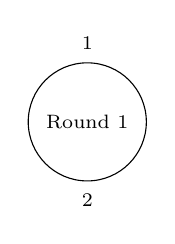
\begin{tikzpicture}[baseline={(current bounding box.north)}, font=\scriptsize]
				\draw[align=center]
				(0,0) circle (0.75) node {Round 1}
				(0,1) node {1}
				(0,-1) node {2}
				;
			\end{tikzpicture}
			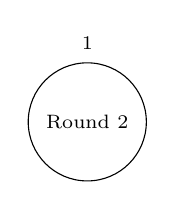
\begin{tikzpicture}[baseline={(current bounding box.north)}, font=\scriptsize]
				\draw[align=center]
				(0,0) circle (0.75) node {Round 2}
				(0,1) node {1}
				;
			\end{tikzpicture} \\
			is true. \\
			\textbf{Inductive hypothesis:} \\
			Assume $P(k): 2^k$ people eliminated as given above will eventually leave only person \#1 for $k\geq1$ is true. \\
			Prove $P(k+1): 2^{k+1}$ people eliminated as given above will eventually leave only person \#1: \\
			After round 1 there are $2^k$ people. \\
			Because $P(k)$ is true, by round 2, when there are $2^k$ people left, carrying out eliminations as given above must leave only person \#1. \\
			Basis and inductive hypothesis proven, therefore original statement is true. \\
		}
	}
	\chunk{
		\set{4}{30}{d}{
			It is a fact that every integer $n\geq1$ can be written in the form  \\
			$c_r\cdot3^r+c_{r-1}\cdot3^{r-1}+\dots+c_2\cdot3^2+c_1\cdot3+c_0$, \\
			where $c_r=1$ or 2 and $c_i=0,1,$ or 2 for all integers $i=0,1,2,\dots,r-1$. Sketch a proof of this fact. \\
			Let property $P(n)$ be the the property given above. \\
			$P(n)$ says that any positive integer can be written as the sum of multiples of powers of 3. \\
			\textbf{Basis:} \\
			$P(1): (c_{r=0}=1)\cdot3^{r=0}=1$ is true. \\
			$P(2): (c_{r=0}=1)\cdot3^{r=0}+(c_0=1)=2$ is true. \\
			$P(3): (c_{r=1}=1)\cdot3^{r=1}=3$ is true. \\
			$P(4): (c_{r=1}=1)\cdot3^{r=1}+(c_{r=0}=1)\cdot3^{r=0}=4$ is true. \\
			\textbf{Inductive hypothesis:} \\
			Let $k\geq4$. \\
			Assume $P(i)$ for $1\leq i\leq k$ and $i\in\mathbb{Z}$ to be true. \\
			Prove $P(k+1)$ can be written as the sum of multiples of powers of 3: \\
			\begin{tabular}{|l|}
				\hline
				\case{1}{$k+1$ mod $3=0$} \\
				\hline
				$\left.\begin{aligned}
					& 1\leq (k+1)/3\leq k \\
					& 2\leq k \leq 3k-1 \\
					& k\geq 2 \\
				\end{aligned}\right\}$ is true. \\
				$\dfrac{k+1}{3}=c_r\cdot3^r+c_{r-1}\cdot3^{r-1}+\dots+c_2\cdot3^2+c_1\cdot3+c_0$ because $P(i)$ \\
				$k+1=c_r\cdot3^{r+1}+c_{r-1}\cdot3^r+\dots+c_2\cdot3^3+c_1\cdot3^2+c_0\cdot3$ \\
				$k+1$ is the sum of multiples of powers of 3. \\
				Proof done. \\
				\hline
				\case{2}{$k+1$ mod $3=1$} \\
				\hline
				$k$ mod $3=0$ \\
				$\left.\begin{aligned}
					& 1\leq k/3\leq k \\
					& 3\leq k\leq 3k \\
					& k\geq 3 \\
				\end{aligned}\right\}$ is true. \\
				$\dfrac{k}{3}=c_r\cdot3^r+c_{r-1}\cdot3^{r-1}+\dots+c_2\cdot3^2+c_1\cdot3+c_0$ because $P(i)$ \\
				$k=c_r\cdot3^{r+1}+c_{r-1}\cdot3^r+\dots+c_2\cdot3^3+c_1\cdot3^2+c_0\cdot3$ \\
				$k+1=c_r\cdot3^{r+1}+c_{r-1}\cdot3^r+\dots+c_2\cdot3^3+c_1\cdot3^2+c_0\cdot3+(1\cdot3^0=1)$ \\
				$k+1$ is the sum of multiples of powers of 3. \\
				Proof done. \\
				\hline
				\case{3}{$k+1$ mod $3=2$} \\
				\hline
				$k-1$ mod $3=0$ \\
				$\left.\begin{aligned}
					& 1\leq (k-1)/3\leq k \\
					& 4\leq k \leq 3k+1 \\
					& k\geq 4 \\
				\end{aligned}\right\}$ is true. \\
				$\dfrac{k-1}{3}=c_r\cdot3^r+c_{r-1}\cdot3^{r-1}+\dots+c_2\cdot3^2+c_1\cdot3+c_0$ because $P(i)$ \\
				$k-1=c_r\cdot3^{r+1}+c_{r-1}\cdot3^r+\dots+c_2\cdot3^3+c_1\cdot3^2+c_0\cdot3$ \\
				$k+1=c_r\cdot3^{r+1}+c_{r-1}\cdot3^r+\dots+c_2\cdot3^3+c_1\cdot3^2+c_0\cdot3+(2\cdot3^0=2)$ \\
				$k+1$ is the sum of multiples of powers of 3. \\
				Proof done. \\
				\hline
			\end{tabular} \\
			$P(k+1)$ is true in all cases. \\
			Basis and inductive hypothesis proven, therefore original statement is true. \\
		}
	}
	\chunk{
		\set{5}{30}{e}{
			$F_0,F_1,F_2,\dots$ is the Fibonacci sequence. \\
			Use mathematical induction to prove that for all integers $n\geq0$, $F_{n+2}F_n-F^2_{n+1}=(-1)^n$ \\
			Let property $P(n)$ be $F_{n+2}F_n-F^2_{n+1}=(-1)^n$. \\
			\textbf{Basis:} \\
			$F_0=1$, $F_1=1$, $F_2=2$ \\
			$P(0): (F_2F_0-F^2_1=2\cdot1-1^2=1)=((-1)^0=1)$ is true. \\
			\textbf{Inductive hypothesis:} \\
			Assume $P(k): F_{k+2}F_k-F^2_{k+1}=(-1)^k$ for $k\geq0\in\mathbb{Z}$ to be true. \\
			Prove $P(k+1): F_{k+3}F_{k+1}-F^2_{k+2}=(-1)^{k+1}$: \\
			$\begin{aligned}[t]
				F_{k+3}F_{k+1}-F^2_{k+2} &= (F_{k+2}+F_{k+1})F_{k+1}-(F_{k+1}+F_{k})^2 \\
				&= (2F_{k+1}+F_k)F_{k+1}-(F^2_{k+1}+2F_{k+1}F_k+F^2_{k}) \\
				&= 2F^2_{k+1}+F_kF_{k+1}-(F^2_{k+1}+2F_{k+1}F_k+F^2_{k}) \\
				&= F^2_{k+1}-F_kF_{k+1}-F^2_k \\
				&= F^2_{k+1}-F_k(F_{k+1}+F_k) \\
				&= F^2_{k+1}-F_kF_{k+2}=-(F_{k+2}F_k-F^2_{k+1})=-(-1)^k=(-1)^{k+1}\\
			\end{aligned}$ \\
			Basis and inductive hypothesis proven, therefore original statement is true. \\
		}
	}
	\chunk{
		\quesa{f}{Let $f$ be a function on whole numbers satisfying}{
			$f(n)=
			\begin{cases}
				0 & \text{if $n=0$} \\
				4f(n/2) & \text{if $n>0$ and even} \\
				f(n-1)+2n-1 & \text{if $n>0$ and odd} \\
			\end{cases}$ \\
			Prove that $f(n)=n^2$ for all $n\geq0$. \\
			Let property $P(n)$ be $f(n)=n^2$. \\
			\textbf{Basis:} \\
			$P(0): (f(0)=0)=(0^2=0)$ is true. \\
			$P(1): (f(0)+2\cdot1-1=1)=(1^2=1)$ is true. \\
			\textbf{Inductive hypothesis:} \\
			Let $k\geq1$. \\
			Assume $P(i): f(i)=i^2$ for $0\leq i\leq k$ and $i\in\mathbb{Z}$ to be true. \\
			Prove $P(k+1): f(k+1)=(k+1)^2$: \\
			\begin{tabular}{|l|}
				\hline
				\case{1}{$k+1$ is even} \\
				\hline
				$\left.\begin{aligned}
					0\leq(k+1)/2\leq k \\
					0\leq k+1\leq2k \\
					-k\leq1\leq k \\
					k\geq1 \\
				\end{aligned}\right\}$ is true. \\
				$\begin{aligned}[t]
					f(k+1) &= 4f((k+1)/2) \\
					&= 4\left(\dfrac{k+1}{2}\right)^2 & \text{$P(i)$ is true} \\
					&= (k+1)^2 \\
				\end{aligned}$ \\
				Proof done. \\
				\hline
			\end{tabular}
			\begin{tabular}{|l|}
				\hline
				\case{2}{$k+1$ is odd} \\
				\hline
				$\left.\begin{aligned}
					0\leq k/2\leq k \\
					0\leq k\leq 2k \\
					-k\leq0\leq k \\
					k\geq0 \\
				\end{aligned}\right\}$ is true. \\
				$\begin{aligned}[t]
					f(k+1) &= f((k+1)-1)+2(k+1)-1 \\
					&= f(k)+2k+1 \\
					&= k^2+2k+1 & \text{$P(i)$ is true} \\
					&= (k+1)^2 \\
				\end{aligned}$ \\
				Proof done. \\
				\hline
			\end{tabular}\\
			Basis and inductive hypothesis proven, therefore original statement is true. \\
		}
	}

	\chunk{
		\problem{3}
		\sets{5}{28, 29}{a}{
			$F_0,F_1,F_2,\dots$ is the Fibonacci sequence. \\
			$F_0=1$, $F_1=1$, $F_2=2$, $F_3=3$
			\begin{enumerate}
				\item [28.]
				Prove that $F^2_{k+1}-F^2_k-F^2_{k-1}=2F_kF_{k-1}$, for all integers $k\geq1$. \\
				Let property $P(n)$ be $F^2_{n+1}-F^2_n-F^2_{n-1}=2F_nF_{n-1}$. \\
				\textbf{Basis:} \\
				$P(1): (F^2_2-F^2_1-F^2_0=2^2-1^2-1^2=2)=(2F_1F_0=2\cdot1\cdot1=2)$ is true. \\
				\textbf{Inductive hypothesis:} \\
				Assume $P(k): F^2_{k+1}-F^2_k-F^2_{k-1}=2F_kF_{k-1}$ for $k\geq1$ to be true. \\
				Prove $P(k+1): F^2_{k+2}-F^2_{k+1}-F^2_k=2F_{k+1}F_k$: \\
				$\begin{aligned}
					F^2_{k+2}-F^2_{k+1}-F^2_k &= (F_{k+1}+F_k)^2-(F_k+F_{k-1})^2-F^2_k \\
					&= (2F_k+F_{k-1})^2-(F_k+F_{k-1})^2-F^2_k \\
					&= 4F^2_k+4F_kF_{k-1}+F^2_{k-1}-(F^2_k+2F_kF_{k-1}+F_{k-1}^2)-F^2_k \\
					&= 2F^2_k+2F_kF_{k-1} \\
					&= 2F_k(F_k+F_{k-1}) \\
					&= 2F_kF_{k+1} \\
				\end{aligned}$ \\
				Basis and inductive hypothesis proven, therefore original statement is true. \\

				\item [29.]
				Prove that $F^2_{k+1}-F^2_k=F_{k-1}F_{k+2}$, for all integers $k\geq1$. \\
				Let property $P(n)$ be $F^2_{n+1}-F^2_n=F_{n-1}F_{n+2}$. \\
				\textbf{Basis:} \\
				$P(1): (F^2_2-F^1_1=3)=(F_0F_3=3)$ is true. \\
				\textbf{Inductive hypothesis:} \\
				Assume $P(k): F^2_{k+1}-F^2_k=F_{k-1}F_{k+2}$ for $k\geq1\in\mathbb{Z}$ to be true. \\
				Prove $P(k+1): F^2_{k+2}-F^2_{k+1}=F_kF_{k+3}$: \\
				$\begin{aligned}[t]
					F^2_{k+2}-F^2_{k+1} &= (F_{k+1}+F_k)^2-(F_k+F_{k-1})^2 \\
					&= (2F_k+F_{k-1})^2-(F^2_k+2F_kF_{k-1}+F^2_{k-1}) \\
					&= 4F^2_k+4F_kF_{k-1}+F^2_{k-1}-(F^2_k+2F_kF_{k-1}+F^2_{k-1}) \\
					&= 3F^2_k+2F_kF_{k-1} \\
					&= F_k(3F_k+2F_{k-1}) \\
					&= F_k(F_{k+1}+2F_k+F_{k-1}) \\
					&= F_k(F_{k+2}+F_k+F_{k-1}) \\
					&= F_k(F_{k+2}+F_{k+1}) \\
					&= F_kF_{k+3} \\
				\end{aligned}$ \\
				Basis and inductive hypothesis proven, therefore original statement is true. \\
			\end{enumerate}
		}
	}
	\chunk{
		\set{6}{2(b,d)}{b}{
			The formula \\
			$1+r+r^2+\dots+r^n=\dfrac{r^{n+1}-1}{r-1}$ \\
			is true for all real numbers $r$ except for $r=1$ and for all integers $n\geq0$.
			\begin{enumerate}
				\item [(b)]
				If $n$ is an integer and $n\geq1$, find a formula for the expression $3^{n-1}+3^{n-2}+\dots+3^2+3+1$. \\
				$\Sum{i=0}{n-1}3^i =\dfrac{3^n-1}{2}$ \\

				\item [(d)]
				If $n$ is an integer and $n\geq1$, find a formula for the expression \\
				$2^n-2^{n-1}+2^{n-2}-2^{n-3}+\dots+(-1)^{n-1}\cdot2+(-1)^n$. \\
				$(-1)^02^n+(-1)^12^{n-1}+(-1)^22^{n-2}+(-1)^32^{n-3}+\dots+(-1)^{n-1}\cdot2^1+(-1)^n2^0$. \\
				$\begin{aligned}[t]
					\Sum{i=0}{n}(-1)^i2^{n-i} &= \Sum{i=0}{n}(-1)^i\dfrac{2^n}{2^i} \\
					&= 2^n\Sum{i=0}{n}\dfrac{(-1)^i}{2^i} \\
					&= 2^n\Sum{i=0}{n}\left(-\dfrac{1}{2}\right)^i \\
					&= 2^n\dfrac{\left(-\frac{1}{2}\right)^{n+1}-1}{-\frac{1}{2}-1} \\
					&= 2^n\dfrac{2((-\frac{1}{2})^{n+1}-1)}{3} \\
					&= -\dfrac{2^{n+1}((-\frac{1}{2})^{n+1}-1)}{3} \\
					&= -\dfrac{(-1)^{n+1}-2^{n+1}}{3} \\
					&= \dfrac{2^{n+1}-(-1)^{n+1}}{3} \\
				\end{aligned}$ \\
			\end{enumerate}
		}
	}
%	\chunk{
	\sets{6}{9, 14, 15}{c}{
		\chunk{
			\ques{9.}{$g_k=\dfrac{g_{k-1}}{g_{k-1}+2}$ for all integers $k\geq2$}{
				$g_1=1$ \\
				$\begin{aligned}[t]
					g_2 &= \dfrac{1}{1+2} = \dfrac{1}{1+2^1}\\
					g_3 &= \dfrac{\frac{1}{1+2}}{\frac{1}{1+2}+2} = \dfrac{1}{1+2}\cdot\dfrac{1+2}{1+2(1+2)} = \dfrac{1}{1+2(1+2)} = \dfrac{1}{1+2^1+2^2} \\
					g_4 &= \dfrac{\frac{1}{1+2+4}}{\frac{1}{1+2+4}+2} = \dfrac{1}{1+2+4}\cdot\dfrac{1+2+4}{1+2(1+2+4)} = \dfrac{1}{1+2(1+2+4)} = \dfrac{1}{1+2^1+2^2+2^3} \\
				\end{aligned}$ \\
				$g_k=\dfrac{1}{\Sum{i=0}{k-1}2^i}$ \\
				$g_k=\dfrac{1}{\dfrac{2^{(k-1)+1}-1}{2-1}}$ \\
				$g_k=\dfrac{1}{2^k-1}$ \\
			}
		}
%		\chunk{
			\newpage
			\ques{14.}{$x_k=3x_{k-1}+k$, for all integers $k\geq2$}{
				$x_1=1$ \\
				$\begin{aligned}[t]
					x_2 &= 3\cdot1+2 \\
					x_3 &= 3(3\cdot1+2)+3 = 3^2\cdot1+3\cdot2+3\\
					x_4 &= 3(3^2\cdot1 + 3\cdot2 + 3)+4 = 3^3\cdot1+3^2\cdot2+3\cdot3+4 \\
				\end{aligned}$ \\
				$x_k=\Sum{i=0}{k-1}3^i(k-i)=\Sum{i=0}{k-1}k3^i-\Sum{i=0}{k-1}i3^i=k\cdot\dfrac{3^k-1}{2}-\Sum{i=1}{k-1}i3^i$ \\
				Let $S=\Sum{i=1}{k-1}i3^i=1\cdot3+2\cdot3^2+\dots+(k-2)3^{k-2}+(k-1)3^{k-1}$ \\
				$\left.\begin{aligned}
					S & {}={} & 3+3^2+\dots+3^{k-2}+3^{k-1} \\
					& & +3^2+\dots+3^{k-2}+3^{k-1} \\
					& & \vdots \\
					& & +3^{k-2}+3^{k-1} \\
					& & +3^{k-1} \\
				\end{aligned}\right\}$ $k-1$ lines \\
				$\begin{aligned}[t]
					S &= \Sum{i=1}{k-1}\Sum{j=i}{k-1}3^j \\
					&= \Sum{i=1}{k-1}\left(\Sum{j=1}{k-1}3^j-\Sum{j=1}{i-1}3^j\right) \\
					&= \Sum{i=1}{k-1}\left(\dfrac{3^k-3}{2}-\dfrac{3^i-3}{2}\right) \\
					&= (k-1)\dfrac{3^k-3}{2}-\Sum{i=1}{k-1}\dfrac{3^i-3}{2} \\
					&= (k-1)\dfrac{3^k-3}{2}-\dfrac{1}{2}\left(\Sum{i=1}{k-1}3^i-3(k-1)\right) \\
					&= (k-1)\dfrac{3^k-3}{2}-\dfrac{1}{2}\Sum{i=1}{k-1}3^i+\dfrac{1}{2}(3k-3) \\
					&= \dfrac{k\cdot3^k-3^k-3k+3}{2}-\dfrac{1}{2}\cdot\dfrac{3^k-3}{2}+\dfrac{3k-3}{2} \\
					&= \dfrac{2k\cdot3^k-2\cdot3^k-6k+6}{4}-\dfrac{3^k-3}{4}+\dfrac{6k-6}{4} \\
%					&= \dfrac{2k\cdot3^k-3^k-2k+1}{4}-\dfrac{4k+4}{4} \\
					&= \dfrac{2k\cdot3^k-3^{k+1}+3}{4} \\
%					&= \dfrac{3^k(2k-1)-3(2k+1)}{4} \\
				\end{aligned}$ \quad
				$\begin{aligned}[t]
					1+r+r^2+\dots+r^n &=\dfrac{r^{n+1}-1}{r-1} \\
					r+r^2+\dots+r^n &=\dfrac{r^{n+1}-1}{r-1}-1 \\
					r+r^2+\dots+r^n &=\dfrac{r^{n+1}-r}{r-1} \\
%					r+r^2+\dots+r^n &=\dfrac{r\left(r^n-1\right)}{r-1} \\
					\Sum{i=1}{n}r^i &=\dfrac{r^{n+1}-r}{r-1} \\
				\end{aligned}$\\
				$x_k=k\cdot\dfrac{3^k-1}{2}-S$ \\
				$x_k=\dfrac{k\cdot3^k-k}{2}-\dfrac{2k\cdot3^k-3^{k+1}+3}{4}$ \\
				$x_k=\dfrac{2k\cdot3^k-2k}{4}-\dfrac{2k\cdot3^k-3^{k+1}+3}{4}$ \\
				$x_k=\dfrac{3^{k+1}-2k-3}{4}$ \\
			}
%		}
		\chunk{
			\ques{15.}{$y_k=y_{k-1}+k^2$, for all integers $k\geq2$}{
				$y_1=1$ \\
				$\begin{aligned}[t]
					y_2 &= 1+2^2 = 5 \\
					y_3 &= (1+2^2)+3^2 = 14 \\
					y_4 &= (1+2^2+3^2)+4^2 = 30 \\
				\end{aligned}$ \\
				$y_k=\Sum{i=1}{k}i^2$ \\
				$\left.\begin{aligned}
					y_k & {}={} & 1+2+3+4+\dots+(k-1)+k \\
					& & {}+2+3+4+\dots+(k-1)+k \\
					& & {}+3+4+\dots+(k-1)+k \\
					& & {}+4+\dots+(k-1)+k \\
					& & \vdots \\
					& & {}+(k-1)+k \\
					& & {}+k \\
				\end{aligned}\right\}$ $k$ lines \\
				$\begin{aligned}[t]
					y_k &= \Sum{i=1}{k}\Sum{j=i}{k}j \\
					&= \Sum{i=1}{k}\left(\Sum{j=1}{k}j-\Sum{j=1}{i-1}j\right) \\
					&= \Sum{i=1}{k}\left(\dfrac{k(k+1)}{2}-\dfrac{i(i-1)}{2}\right) \\
					&= k\cdot\dfrac{k(k+1)}{2}-\Sum{i=1}{k}\dfrac{i(i-1)}{2} \\
					&= \dfrac{k^2(k+1)}{2}-\Sum{i=1}{k}\left(\dfrac{i^2}{2}-\dfrac{i}{2}\right) \\
					&= \dfrac{k^2(k+1)}{2}+\Sum{i=1}{k}\dfrac{i}{2}-\Sum{i=1}{k}\dfrac{i^2}{2} \\
					&= \dfrac{k^2(k+1)}{2}+\dfrac{1}{2}\Sum{i=1}{k}i-\dfrac{1}{2}\Sum{i=1}{k}i^2 \\
				\end{aligned}$ \\
				$\begin{aligned}[t]
					y_k &= \dfrac{k^2(k+1)}{2}+\dfrac{1}{2}\cdot\dfrac{k(k+1)}{2}-\dfrac{1}{2}y_k \\
					4y_k &= 2k^2(k+1)+k(k+1)-2y_k \\
					6y_k &= (k+1)(2k^2+k) \\
					y_k &= \dfrac{k(k+1)(2k+1)}{6} \\
				\end{aligned}$
			}
		}
	}
\end{document}